\documentclass[nobib]{tufte-handout}

\title{Lecture 6: Weights, distances, and minimum spanning trees $\cdot$ 1MA020}

\author[Vilhelm Agdur]{Vilhelm Agdur\thanks{\href{mailto:vilhelm.agdur@math.uu.se}{\nolinkurl{vilhelm.agdur@math.uu.se}}}}

\date{10 November 2023}


%\geometry{showframe} % display margins for debugging page layout

\usepackage{graphicx} % allow embedded images
  \setkeys{Gin}{width=\linewidth,totalheight=\textheight,keepaspectratio}
  \graphicspath{{graphics/}} % set of paths to search for images
\usepackage{amsmath}  % extended mathematics
\usepackage{booktabs} % book-quality tables
\usepackage{units}    % non-stacked fractions and better unit spacing
\usepackage{multicol} % multiple column layout facilities
\usepackage{lipsum}   % filler text
\usepackage{fancyvrb} % extended verbatim environments
  \fvset{fontsize=\normalsize}% default font size for fancy-verbatim environments

\usepackage{color,soul} % Highlights for text

% Standardize command font styles and environments
\newcommand{\doccmd}[1]{\texttt{\textbackslash#1}}% command name -- adds backslash automatically
\newcommand{\docopt}[1]{\ensuremath{\langle}\textrm{\textit{#1}}\ensuremath{\rangle}}% optional command argument
\newcommand{\docarg}[1]{\textrm{\textit{#1}}}% (required) command argument
\newcommand{\docenv}[1]{\textsf{#1}}% environment name
\newcommand{\docpkg}[1]{\texttt{#1}}% package name
\newcommand{\doccls}[1]{\texttt{#1}}% document class name
\newcommand{\docclsopt}[1]{\texttt{#1}}% document class option name
\newenvironment{docspec}{\begin{quote}\noindent}{\end{quote}}% command specification environment

\include{mathcommands.extratex}

\begin{document}

\maketitle% this prints the handout title, author, and date

\begin{abstract}
\noindent
Continuing from our previous discussion on the existence of spanning trees and counting of them, we come to the problem of actually finding them. We give two different algorithms for this. Finally we consider the problem of computing distances in a graph, and give an algorithm for this.
\end{abstract}

As we saw in the exercises in our previous session, the question of spanning trees becomes more interesting if we also add weights to the edges of our graph, since we can then consider the \emph{minimum} spanning trees.

We also saw that to do this, we need to restrict ourselves to finite graphs,\sidenote[][]{Later, when we measure distances, we will also need to assume all weights are positive, or we will again have silly things happen.} or stupid things will happen. If we additionally assume that all weights are distinct, there is even a \emph{unique} minimal spanning tree.

\section{Prim's algorithm}

The first algorithm we introduce for this is Prim's algorithm, which works by starting in a particular vertex and growing the tree.

\begin{figure}
  \centering
  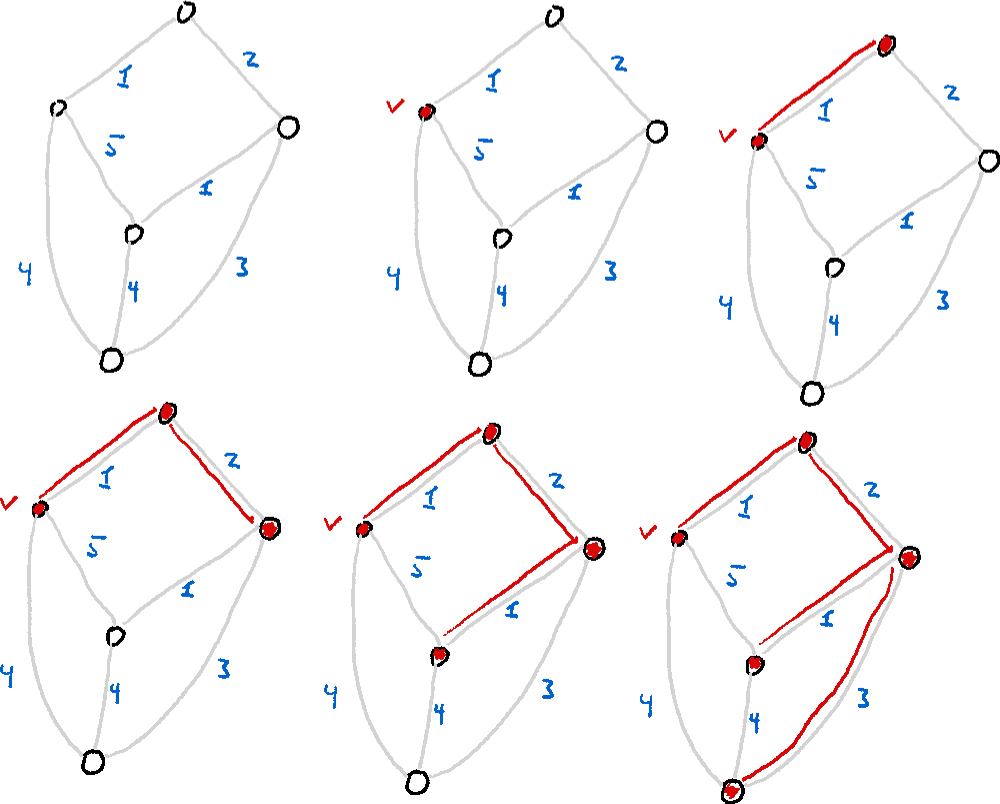
\includegraphics[width=0.85\textwidth]{graphics/L6_prim_kruskal_dijkstra/prims_algorithm.png}
  \caption[][0cm]{An illustration of how Prim's algorithm finds a minimal spanning tree in a graph.}
  \label{fig:prims_algorithm}
\end{figure}

\begin{definition}[Prim's algorithm]
  Let $G = (V,E,w)$ be a finite connected weighted graph, and let $v \in V$ be an arbitrary vertex of $G$. Initialize the algorithm by setting $T = (\{v\}, \emptyset)$, the subtree containing only $v$.

  As long as $T$ is not a spanning subgraph, find an edge $e$ of $G$ between $V(T)$ and $V(T)^c$ which has minimal weight. Add this edge together with its endpoint in $V(T)^c$ to $T$. When $V(T) = V$, return $T$.

  How this algorithm constructs an MST is illustrated in Figure \ref{fig:prims_algorithm}.
\end{definition}

Before we can prove that this algorithm actually works, we will need a little lemma about what happens when you remove edges from trees.\sidenote[][]{This statement is perhaps in some sense obvious, but it did not occur to me immediately. The proof in the old lecture notes omits the steps that would even require the lemma, and the proofs I found online did not omit those steps but did leave the lemma implicit.}

\begin{lemma} \label{lemma:removing_edges_from_trees}
  If $T = (V, E)$ is a tree and $e = (u, w)$ an edge of $T$, then $F = (V, E \setminus e)$, the graph gotten by removing the edge $e$ from $T$, has exactly two connected components, both of which are trees.

  More generally, removing $k$ edges from a tree will create $k+1$ connected components, each of which is a tree.
  
  \begin{proof}
    That the connected components of a graph gotten by removing edges from a tree will always be trees is easy to see -- they are by definition connected, and removing edges can't have introduced any cycles, so they are connected and acyclic, i.e. trees.\sidenote[][]{A graph all of whose connected components are trees is called a \emph{forest}, of course. These are precisely the acyclic graphs. So one very poor definition of ``tree'' could be ``a tree is a connected forest''.}

    Now, to see that $F$ must have exactly two connected components, let $U$ be the connected component containing $u$, and likewise for $W$. Assume $v$ is some vertex not in $U$ -- we will show it is then in $W$.

    Since $T$ is connected, there is a path $P$ connecting $v$ to $u$ -- and since $v$ is not in $U$, this path must have been destroyed by removing the edge $e$. Now, since $e = (w, u)$ is incident to $u$, it must in fact have been the final edge of the path $P$, so we can write
    $$P = v\, e_1\, v_1\, e_2\, \ldots\, e_\ell\, w\, e\, u.$$
    
    This however means that by removing the last edge of $P$ we get a path from $v$ to $w$, proving that $v \in W$, as desired.

    The result for a general number of edges removed follows by induction from the one-edge case.
  \end{proof}
\end{lemma}

\begin{theorem}
  Prim's algorithm is correct, that is, it always generates a minimum spanning tree.

  \begin{proof}
    Let $G = (V,E,w)$ be a finite connected weighted graph, and let the sequence of subgraphs that Prim's algorithm creates be $T_0 \subseteq T_1 \subseteq \ldots \subseteq T_{n-1} = T$. It is easy to see that $T_i$ will always be connected and have $i$ edges, so $T_{n-1}$ has to be a tree, so Prim's algorithm at least always finds \emph{a} spanning tree.
    
    To see that this spanning tree is minimal, we consider an MST $T'$, and show that $w(T) \leq w(T')$. If $T = T'$ we are done, so assume they are distinct, and let
    $$j = \max\left\{i \in \{0,1,\ldots,n-1\} \given T_i \subseteq T'\right\}.$$
    That is, $j$ is the final time at which all edges of $T_j$ are also edges of $T'$.

    So, let $e = (u, w)$ be the edge between $V(T_j)$ and $V(T_j)^c$ added by the next step of the algorithm, with $u \in V(T_j)$ and $w \in V(T_j)^c$. By assumption, this edge is not in $T'$.
    
    Since $T'$ is a tree, there must be a unique path in $T'$ connecting $u$ and $w$, and at some point this path must cross from $V(T_j)$ into $V(T_j)^c$. Call the edge it crosses with $f = (u', w')$.

    By construction, $e$ has minimal weight among all edges between $V(T_j)$ and $V(T_j)^c$, so we must have $w(e) \leq w(f)$. Let us now show that we can modify the tree $T'$ into a different spanning tree $T''$ which contains $e$ and satisfies $w(T'') \leq w(T')$, so that $T''$ is also an MST.

    The way we do this is of course by removing the edge $f$ from $T'$ and adding the edge $e$. It is clear that this does not increase the weight of the graph, so the thing we need to show is that it is still a tree. 
    
    It follows from Lemma \ref{lemma:removing_edges_from_trees} that removing the edge $f$ yields a graph with two connected components, $V(T_j)$ and $V(T_j)^c$, each of which is a tree. Clearly the edge $e$ also goes between these components, so adding it back in will reconnect the two trees, and that adding an edge between two disconnected trees yields a tree is clear, since it connects the graph and can't possibly add a cycle.

    So we can repeat this process inductively, taking the new tree $T''$ as the new MST with which we compare $T$, until eventually $T = T^{'''\cdots'''}$ and so $T$ is an MST.
  \end{proof}
\end{theorem}

\begin{remark}
  The runtime of this algorithm will depend on the implementation -- specifically on how the graph is represented\sidenote[][-0.9cm]{Are you storing essentially an adjacency matrix, or a list of edges, or something like a ``linked list'' kind of structure? There are many ways of representing a graph in memory.} and on how you find the next edge between $V(T_i)$ and $V(T_i)^c$. A good implementation has a runtime of $O\left(\abs{E} + \abs{V}\log\left(\abs{V}\right)\right)$.\sidenote[][]{If you just store an adjacency matrix, you get a runtime of $O\left(\abs{V}^2\right)$, while if you store the graph as a list of vertices, where each vertex is a list of its neighbours, and use a Fibonacci heap to help finding the minimal edges, you get the runtime of the ``good'' implementation.}
\end{remark}

\section{Exercises}

%\bibliography{references}
%\bibliographystyle{plainnat}

\end{document}
